
\section{Results \& discussion}\label{sec:results_discussion}

To test the devised simulation, we ran a series of simulations in Trindade, a major station in Porto's metro system (Portugal). \autoref{fig:trindade} \\

\begin{figure}
    \centering
    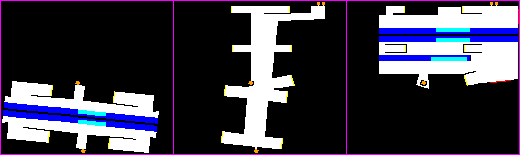
\includegraphics[width=\linewidth]{assets/trindade.png}
    \caption{Map for Trindade's station in NetLogo}
    \label{fig:trindade}
\end{figure}

We ran the following scenarios:

\begin{itemize}
    \item Normal
    \item No elevators
    \item Only one set of stairs per train
    \item Longer trains
    \item With escalators
\end{itemize}

For each scenario, we ran with a passenger load of 150 and 300. The metrics collected are listed below. In \autoref{sec:annexes} all of the tables with the metrics by experiment are listed. For each metric, a simple statistical analysis was performed.
\begin{itemize}
    \item Number of ticks: The number of ticks that it takes to run the experiment and for every passenger to reach their destination \ref{annex:tick}
    \item Distance per tick: The distance a passenger travels in a tick. By definition should be 0.3 units \ref{annex:tick_distance}
    \item Total distance: The total distance traveled by a passenger to reach their destination.  \ref{annex:distance}
    \item Crowdedness: The number of other passengers inside the given radius. \ref{annex:crowdedness_0.8}, \ref{annex:crowdedness_1}, \ref{annex:crowdedness_1.2}, \ref{annex:crowdedness_1.4}
\end{itemize}

When analysing the number of ticks of each experiment, we can see that not always does the experiment of 300 passengers take more steps to run. Additionally, the scenarios with no elevators or a single set of stairs do increase the number of ticks, as expected, since passengers will not always be able to take what would otherwise be the shortest path. There doesn't seem to be a great difference between the base scenario and the scenario with escalators, which leads us to conclude that maybe the shortest path does not include the escalators. (or if it does, there is no significant benefit). One thing to notice is that there seems to have been some abnormal behavior in experiments \textit{trindade-300} and \textit{trindade-single-stairs} as is seen by the \textit{max} column, which presents a much higher value. The percentiles are still within reason so we can interpret those values as outliers.

When it comes to the tick distance, the \textit{max} column is where we should focus on. A tick distance higher than 0.3 happens when the collision mechanisms push a passenger out of the way. A 75th percentile of 0.3 is therefore expected as collisions are not that frequent. The higher number of passengers and scenarios with less pathing alternatives leading to an, even if slight, increase in the maximum amount is expected but inconclusive. To be certain, we'd need to have higher percentiles of the data to see if this relation holds not only for the tick with the maximum distance, but for the ticks that employ some collision mechanism.

When it comes to totally distance travelled, mean values for each scenario are according to the hypothesis that less available pathing alternatives lead to worse outcomes. The scenarios \textit{trindade}, \textit{trindade-long-trains}, and \textit{trindade-escalators} having the same paths available have a similar mean distance traveled, where as \textit{trindade-no-elevators} has a higher distance traveled, and \textit{trindade-single-stairs} higher even. Looking in particular at the scenario with single stairs, there is a 100 units difference between the experiment with 150 and 300 passengers. This distance could be explained by a worse starting position for a passenger. One thing to notice is that there is an almost perfect correlation between total distance and number of ticks. As such, referring back to the maximum value for the number of ticks in the \textit{trindade-300} experiment which isn't reflected in the maximum distance traveled, we could hypothesize that that passenger might have become stuck, maybe as a malfunctioning of the simulation.

When it comes to crowdedness metrics, we can see that the numbers for the experiments with double the number of passengers are more or less double that of the normal amount. This is to be expected. The metrics for the scenario with the long trains is significantly lower, which makes sense considering the starting positions of the passengers will be more spaced out. There appears to be little correlation between the other scenarios and the crowdedness otherwise, which could indicate that the starting position of the passengers is the critical criteria for the crowdedness of the experiment. The results for a crowdedness of 0.6 are mostly 0, meaning the radius is too low to obtain any relevant information.

We can see how the differences in the scenarios did not always reflect in the data as would be expected from intuition. This could mean that the simulation is not a truthful interpretation of the real world or that the scenarios presented present insights into the dynamics of people in a transit station.





% \begin{table*}
% \begin{tabular}{|c|c|c|c|cccc|}
% \hline
% \multirow{2}{*}{\textbf{Metric}} & \multirow{2}{*}{\textbf{Ticks}} & \multirow{2}{*}{\textbf{Tick Distance}} & \multirow{2}{*}{\textbf{Total Distance}} & \multicolumn{4}{c|}{\textbf{Crowdedness}}                                                                                \\ \cline{5-8} 
%                                  &                                 &                                         &                                          & \multicolumn{1}{c|}{\textbf{0.8}} & \multicolumn{1}{c|}{\textbf{1.0}} & \multicolumn{1}{c|}{\textbf{1.2}} & \textbf{1.4} \\ \hline
% mean                             & 464.710000                      & 0.297951                                & 138.460790                               & \multicolumn{1}{c|}{0.001160}     & \multicolumn{1}{c|}{0.203689}     & \multicolumn{1}{c|}{0.397329}     & 0.457151     \\ \hline
% std                              & 204.348647                      & 0.024352                                & 61.119533                                & \multicolumn{1}{c|}{0.039845}     & \multicolumn{1}{c|}{0.541747}     & \multicolumn{1}{c|}{0.739537}     & 0.799496     \\ \hline
% min                              & 127.000000                      & 0.000000                                & 38.504057                                & \multicolumn{1}{c|}{0.000000}     & \multicolumn{1}{c|}{0.000000}     & \multicolumn{1}{c|}{0.000000}     & 0.000000     \\ \hline
% 25\%                             & 256.750000                      & 0.300000                                & 76.022187                                & \multicolumn{1}{c|}{0.000000}     & \multicolumn{1}{c|}{0.000000}     & \multicolumn{1}{c|}{0.000000}     & 0.000000     \\ \hline
% 50\%                             & 479.000000                      & 0.300000                                & 141.865455                               & \multicolumn{1}{c|}{0.000000}     & \multicolumn{1}{c|}{0.000000}     & \multicolumn{1}{c|}{0.000000}     & 0.000000     \\ \hline
% 75\%                             & 608.750000                      & 0.300000                                & 182.623531                               & \multicolumn{1}{c|}{0.000000}     & \multicolumn{1}{c|}{0.000000}     & \multicolumn{1}{c|}{1.000000}     & 1.000000     \\ \hline
% Max                              & 898.000000                      & 0.564923                                & 268.083006                               & \multicolumn{1}{c|}{3.000000}     & \multicolumn{1}{c|}{5.000000}     & \multicolumn{1}{c|}{6.000000}     & 6.000000     \\ \hline
% \end{tabular}
% \caption{Obtained results}
% \label{table:results}
% \end{table*}